\documentclass[12pt]{article}

\usepackage[margin=1in]{geometry}
\usepackage{amsmath,amsthm,amssymb}
\usepackage{nccmath}
\usepackage{mathtools}
\usepackage{mathrsfs}
\usepackage{enumitem}
\usepackage{physics}
\usepackage{tensor}

\usepackage{tikz}
\usetikzlibrary{calc,decorations.markings,patterns}

\newcommand{\magsq}[1]{\big|#1\big|^2}
\newcommand{\avg}[1]{\left<#1\right>}
\newcommand{\fullint}{\int_{-\infty}^\infty}
\newcommand{\fullintd}[1]{\fullint\dd#1\:}
\newcommand{\cint}[2]{\int_{#1}^{#2}}
\newcommand{\cintd}[3]{\cint{#1}{#2}\dd#3\:}
\newcommand{\boostXY}{\mqty(\gamma & -\gamma\beta_x & -\gamma\beta_y & 0 \\ -\gamma\beta_x & 1 + (\gamma - 1)\frac{\beta_x^2}{\abs{\beta}^2} & (\gamma - 1)\frac{\beta_x\beta_y}{\abs{\beta}^2} & 0 \\ -\gamma\beta_y & (\gamma - 1)\frac{\beta_x\beta_y}{\abs{\beta}^2} & 1 + (\gamma - 1)\frac{\beta_y^2}{\abs{\beta}^2} & 0 \\ 0 & 0 & 0 & 1)}
\newcommand{\metric}{\mqty(1 & 0 & 0 & 0 \\ 0 & -1 & 0 & 0 \\ 0 & 0 & -1 & 0 \\ 0 & 0 & 0 & -1)}

\begin{document}

\title{Homework 1}
\author{Sean Ericson \\ Phys 661}
\maketitle

\section*{Problem 1}
\begin{enumerate}[label=(\alph*)]
    \item The norm of a four-velocity is given by
    \begin{align*}
        u^\mu u_\mu &= \pdv{x^\mu}{\tau}\pdv{x_\mu}{\tau} \\
        &= \eta_{\mu\nu}\pdv{x^\mu}{\tau}\pdv{x^\nu}{\tau} \\
        &= -\left(\pdv{t}{\tau}\right)^2 + \left(\pdv{x}{\tau}\right)^2 +  \left(\pdv{y}{\tau}\right)^2 + \left(\pdv{z}{\tau}\right)^2 \\
        &= -\gamma^2 + \gamma^2(v_x^2 + v_y^2 + v_z^2) \\
        &= \frac{-1}{1-v^2} + \frac{v^2}{1-v^2} \\
        &= \frac{v^2 - 1}{1 - v^2} \\
        &= -1,
    \end{align*}
    where
    \[ \pdv{t}{\tau} = \gamma; \quad \pdv{x^i}{\tau} = \gamma v_i \]
    was used between the third and fourth lines. Clearly, the zero component of the four-velocity is $\gamma > 0$.

    \item The fact that for any timelike vector there exists a frame in which that vector has zero spatial components is most easily illustrated with a spacetime diagram as in Figure \ref{fig1}. Timelike vectors reside in the future and past light cones. The effect of a boost on the spacetime diagram is to `rotate' the $x$ and $t$ axes into each other. For any line through the origin with slope between -1 and 1, a boost can put the $t$ axis on that line, and in the boosted frame all events on the $t$ axis have zero spatial component. All points in the future/past light cones lie on lines through the origin with slope between -1 and 1, so there exists a boost that takes their spatial components to zero. Mathematically, 
    \[ x' = \gamma(x - vt) = 0 \implies v = \frac{x}{t}, \]
    where $\abs{x/t} < 1$ by the fact that the vector is timelike.
    \begin{figure}
        \centering
        \resizebox{250pt}{!}{
            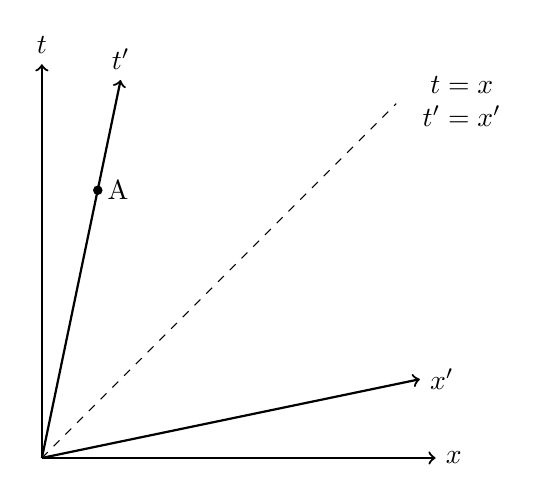
\begin{tikzpicture}
                % Unprimed Axes
                \draw[->, thick] (0,0)--(0,5) node[above]{$t$};
                \draw[->, thick] (0,0)--(5,0) node[right]{$x$};

                % Primed Axes
                \draw[->, thick] (0,0)--(1, 4.8) node[above]{$t'$};
                \draw[->, thick] (0,0)--(4.8, 1) node[right]{$x'$};
        
                % Null line
                \draw[dashed] (0,0)--(4.5,4.5) node[above,right]{\begin{tabular}{c} $t=x$ \\ $t'=x'$ \end{tabular}};

                % Event
                \filldraw (0.71,3.4) circle[radius=1.5pt];
                \node[above, right] at (0.71,3.4) {A};

            \end{tikzpicture}
        }
        \caption{A spacetime diagram illustrating a timelike event which occurs at $x' = 0$.}
        \label{fig1}
    \end{figure}

    \item Let $V^\mu V_\mu > 0$, $W^\mu W_\mu > 0$, and $V^\mu W_\mu = 0$. Then,
    \begin{align*}
        (V+W)^\mu (V+W)_\mu &= V^\mu V_\mu + W^\mu W_\mu + 2V^\mu W_\mu \\
        &= V^\mu V_\mu + W^\mu W_\mu \\
        & > 0
    \end{align*}

    \item Let $A$ be a nonzero timelike vector, and let $B$ be a nonzero null vector. Then, by the result of part (b), there exists a frame in which we can write these vectors as
    \[ A^\mu = (t', 0, 0, 0), \quad B^\mu = (t, x, y, z) \quad (x^2 + y^2 + z^2 = t^2), \] with both $t$ and $t'$ nonzero. Assume for the sake of contradiction that their inner product vanishes. Then,
    \begin{alignat*}{3}
        &          & A^\mu B_\mu = 0 \\
        &\implies  & tt' = 0,
    \end{alignat*}
    thus either $t=0$ or $t'=0$, a contradiction.
\end{enumerate}


\section*{Problem 2}
The magnitude of the centrifugal force is given by
\[ \abs{F_c} = m_I R \omega^2 \sin\theta, \]
where $R$ is the radius of the Earth, $\omega$ is the Earth's rotational velocity, and $\theta$ is the polar angle. For the purpose of the E{\"o}tv{\"o}s experiment, we want to maximize the component of the centrifugal force parallel to the ground (i.e. perpendicular to $\hat{r}$). The maximum value of this component is just the magnitude times $\cos\theta$, so we need to maximize $\sin\theta\cos\theta$, which occurs at $\boxed{\theta = \pi/4}$. The $45^\text{th}$ parallel(s) is(are) the best place(s) to do the experiment, then.

\section*{Problem 3}
\begin{enumerate}[label=(\alph*)]
    \item
    \begin{align*}
        S &= -m\int\dd\tau + q\int\dd x^\mu A_\mu(x) \\
        &= -m\int\sqrt{-\eta_{\mu\nu}\dd x^\mu \dd x^\nu} + q\int\dd x^\mu A_\mu(x) \\
        &= \int\dd\lambda \left[ -m\sqrt{-\eta_{\mu\nu}\dv{x^\mu}{\lambda}\dv{x^\nu}{\lambda}} + qA_\mu(x)\dv{x^\mu}{\lambda} \right]
    \end{align*}

    \item Let $\dot{x}^\mu \coloneqq \dv{x^\mu}{\lambda}$. We can write the action above as the integral of a Lagrangian,
    \[ S = \int\dd\lambda\; L(x, \dot{x}), \]
    where
    \[ L(x, \dot{x}) = -m\sqrt{-\eta_{\mu\nu}\dot{x}^\mu\dot{x}^\nu} + qA_\mu(x)\dot{x}^\mu.\]
    The canonical momentum is given by
    \begin{align*}
        p_\mu &= \pdv{L}{\dot{x}^\mu} \\
        &= m\frac{\dot{x}_\mu}{\sqrt{-\eta_{\alpha\beta}\dot{x}^\alpha\dot{x}^\beta}} + qA_\mu(x) \\
        &= m\frac{\pdv{x_\mu}{\tau}\pdv{\tau}{\lambda}}{\sqrt{-\eta_{\alpha\beta}\pdv{x^\alpha}{\tau}\pdv{x^\beta}{\tau}}\pdv{\tau}{\lambda}} \\
        &= m\frac{u_\mu}{-u\cdot u} + qA_\mu(x) \\
        &= mu_\mu + qA_\mu(x)
    \end{align*}

    \item The Euler-Lagrange equation is
    \[ \dv{\lambda}\pdv{L}{\dot{x}^\mu} = \pdv{L}{x^\mu}. \]
    Note that the left hand side is already $\dv{\lambda} p_\mu$. The only $x^\mu$ dependence is in the gauge filed term,
    \[ \pdv{L}{x^\mu} = q\pdv{A_\nu}{x^\mu}\dot{x}^\nu. \]
    Then, after relabeling indices,
    \[ \dv{p_\mu}{\lambda} = q\pdv{A_\mu}{x^\gamma}\pdv{x^\mu}{\lambda}. \]

    \item 
    \begin{alignat*}{3}
        &         \quad & \dv{p_\mu}{\lambda} &= q\pdv{A_\mu}{x^\gamma}\pdv{x^\mu}{\lambda} \\
        &\implies \quad & \dv{\lambda}\left(mu_\gamma + qA_\gamma\right) &= q\pdv{A_\mu}{x^\gamma}\pdv{x^\mu}{\lambda}   \\
        &\implies \quad & m\dv{u_\gamma}{\lambda} + q\pdv{A_\gamma}{x^\mu}\pdv{x^\mu}{\lambda} & = q\pdv{A_\mu}{x^\gamma}\pdv{x^\mu}{\lambda} \\
        &\implies \quad & m\dv{u_\gamma}{\lambda} &= q\left(\pdv{A_\mu}{x^\gamma}\pdv{x^\mu}{\lambda} - \pdv{A_\gamma}{x^\mu}\pdv{x^\mu}{\lambda}\right) \\
        &\implies \quad & m\dv{u_\gamma}{\tau}\pdv{\tau}{\lambda} &= qF_{\gamma\mu}\pdv{x^\mu}{\tau}\pdv{\tau}{\lambda}  \\
        &\implies \quad & m\dv{u_\gamma}{\tau} &= qF_{\gamma\mu}u^\mu \\
    \end{alignat*}

    \item The antisymmetry of $F_{\gamma\mu}$ is clear from its definition:
    \[ F_{\mu\gamma} = \partial_\mu A_\gamma - \partial_\gamma A_\mu = -(\partial_\gamma A_\mu - \partial_\mu A_\gamma) = -F_{\gamma\mu}. \]
    To check its transformation properties, we first note that under the transformation
    \[ x \to x' = \Lambda x, \]
    the field $A(x)$ transforms as
    \[ A \to A' = \Lambda A(\Lambda^{-1}x). \]
    Then,
    \begin{align*}
        F_{\mu\nu}' &= \pdv{A_\nu'}{x'^\mu} - \pdv{A_\mu'}{x'^\nu} \\
        &= \Lambda_{\;\nu}^\alpha\pdv{A_\alpha}{x'^\mu} - \Lambda_{\;\mu}^{\beta}\pdv{A_\beta}{x'^\nu} \\
        &= \Lambda_{\;\nu}^\alpha\pdv{A_\alpha}{x^\gamma}\pdv{x^\gamma}{x'^\mu} - \Lambda_{\;\mu}^\beta\pdv{A_\beta}{x^\gamma}\pdv{x'^\gamma}{x^\nu} \\
        &= \Lambda_{\;\nu}^\alpha\Lambda_{\;\mu}^\gamma\pdv{A_\alpha}{x^\gamma} - \Lambda_{\;\mu}^\beta\Lambda_{\;\nu}^\gamma\pdv{A_\beta}{x^\gamma} \\
        &= \Lambda_{\;\nu}^\alpha\Lambda_{\;\mu}^\gamma F_{\alpha\gamma},
    \end{align*}
    where in the last step the dummy index $\beta$ was relabeled to $\alpha$. The field strength tensor therefore has the correct transformation properties.

    \item The Lorentz force law gives the force on a charge particle from electric and magnetic fields as
    \[ \vec{F} = q\left(\vec{E} + \vec{v}\times\vec{B}\right). \]
    In components, this is
    \begin{align*}
        F_x &= q\left(E_x + v_yB_z - v_zB_y\right) \\
        F_y &= q\left(E_y + v_zB_x - v_xB_z\right) \\
        F_z &= q\left(E_z + v_xB_y - v_yB_x\right)
    \end{align*}
    The result of part (d) gives mass times proper acceleration as equal to the field strength tensor times the four-velocity,
    \[ ma_\mu = q F_{\mu\nu}u^\nu = q\mqty(F_{00}&F_{01}&F_{02}&F_{03}\\F_{10}&F_{11}&F_{12}&F_{13}\\F_{20}&F_{21}&F_{22}&F_{23}\\F_{30}&F_{31}&F_{32}&F_{33})\mqty(1\\v_x\\v_y\\v_z), \]
    where the four-velocity has been expressed as that of a slow-moving particle. Comparing to the Lorentz force law, we can see that the rows $F_{1i}$, $F_{2i}$, and $F_{3i}$ must be
    \[ \mqty(E_x&0&B_z&-B_y\\E_y&-B_z&0&B_x\\E_z&B_y&-B_x&0). \]
    The antisymmetry of $F$ (and the lack of any constant terms in the force law) then fixes the $0^{th}$ row:
    \[ F_{\mu\nu} = \mqty(0&-E_x&-E_y&-E_z\\E_x&0&B_z&-B_y\\E_y&-B_z&0&B_x\\E_z&B_y&-B_x&0) \]

    \item
    \begin{align*}
        F_{10} &= E_x = \pdv{A_0}{x} - \pdv{A_1}{t} = \left(-\vec{\nabla}\phi - \pdv{\vec{A}}{t}\right)_x \\
        F_{23} &= B_x = \pdv{A_z}{y} - \pdv{A_y}{z} = (\vec{\nabla}\times\vec{A})_x
    \end{align*}
    These are consistent with the usual definitions of the fields in terms of the electrostatic and vector potentials,
    \[ \vec{B} = \vec{\nabla}\times\vec{A}; \quad \vec{E} = -\vec{\nabla}\phi - \pdv{\vec{A}}{t}, \]
    given that $A^0$ is the electrostatic potential $\phi$ (and hence $A_0 = -\phi$).
\end{enumerate}

\end{document}